\documentclass[final]{beamer}

\usetheme{RJH}
\usepackage[utf8]{inputenc}
\usepackage[frenchb]{babel}
\usepackage[orientation=landscape,size=a2,scale=1.2]{beamerposter}
\usepackage[absolute,overlay]{textpos}
\usepackage{url}

\usepackage{graphicx}
\usepackage{color}
\usepackage{hyperref}
\usepackage{amsmath}
\usepackage{amssymb}
\usepackage{pifont}
\newcommand{\cmark}{\ding{51}}%
\newcommand{\xmark}{\ding{55}}%
\usepackage[labelformat=empty]{caption}
\usepackage{framed}
\usepackage{wrapfig}

\setlength{\TPHorizModule}{\paperwidth}
\setlength{\TPVertModule}{\paperheight}

\newcommand{\qedwhite}{\hfill \ensuremath{\Box}}

\definecolor{lightgreen}{rgb}{0.0,0.8,0.0}
\definecolor{lightblue}{rgb}{0.3,0.8,1.0}
\definecolor{lightred}{rgb}{0.874,0.180,0.105}
\definecolor{gray}{rgb}{0.4,0.4,0.4}
\definecolor{lightgray}{rgb}{0.8,0.8,0.8}
\definecolor{shadecolor}{rgb}{0.9,0.9,0.9}

\title{Simple connectome inference from partial correlation statistics in calcium imaging}
\author{Antonio Sutera, Arnaud Joly, Vincent François-Lavet, Zixiao Aaron Qiu, Gilles Louppe, Damien Ernst and Pierre Geurts\\[1.5ex]
{\tiny

\includegraphics[scale=0.16]{images/mail.png}~\url{a.sutera@ulg.ac.be}
%
\includegraphics[scale=0.6]{images/twitter.png}~\href{https://twitter.com/glouppe}{@glouppe}

\includegraphics[scale=0.18]{images/github.png}~\url{https://github.com/asutera/kaggle-connectomics}
}}

\footer{}
\date{}

\makeatletter
\newcommand{\superimpose}[2]{%
  {\ooalign{$#1\@firstoftwo#2$\cr\hfil$#1\@secondoftwo#2$\hfil\cr}}}
\makeatother

\begin{document}
\begin{frame}{}


%% Column 1 ==================================================================

\begin{textblock}{0.32}(0.01,0.14)

%% Signal processing ---------------------------------------------------------

\begin{block}{Signal processing \phantom{p}}

Despite growing interest and practical use in various scientific areas, \textbf{variable
importances derived from tree-based ensemble methods are not well understood
from a theoretical point of view}. In this work we characterize the Mean Decrease
Impurity (MDI) variable importances as measured by an ensemble of totally
randomized trees in asymptotic sample and ensemble size conditions. \textbf{We derive a
three-level decomposition of the  information jointly provided by all input
variables about the output in terms of
\begin{itemize}
\item[] {\color{lightgreen}i) the MDI importance of each input variable,}
\item[] {\color{lightblue}ii) the degree of interaction of an input variable with the other input variables,}
\item[] {\color{lightred}iii) the different interaction terms of a given degree.}
\end{itemize}}
We then
show that this MDI importance of a variable is equal to zero if and only if the
variable is irrelevant and that the MDI importance of a relevant variable is
invariant with respect to the removal or the addition of irrelevant variables.
We illustrate these properties on a simple example and discuss how they may
change in the case of  non-totally randomized trees such as Random Forests and
Extra-Trees.

\vspace{2.5cm}

Despite growing interest and practical use in various scientific areas, \textbf{variable
importances derived from tree-based ensemble methods are not well understood
from a theoretical point of view}. In this work we characterize the Mean Decrease
Impurity (MDI) variable importances as measured by an ensemble of totally
randomized trees in asymptotic sample and ensemble size conditions. \textbf{We derive a
three-level decomposition of the  information jointly provided by all input
variables about the output in terms of
\begin{itemize}
\item[] {\color{lightgreen}i) the MDI importance of each input variable,}
\item[] {\color{lightblue}ii) the degree of interaction of an input variable with the other input variables,}
\item[] {\color{lightred}iii) the different interaction terms of a given degree.}
\end{itemize}}
We then
show that this MDI importance of a variable is equal to zero if and only if the
variable is irrelevant and that the MDI importance of a relevant variable is
invariant with respect to the removal or the addition of irrelevant variables.
We illustrate these properties on a simple example and discuss how they may
change in the case of  non-totally randomized trees such as Random Forests and
Extra-Trees.

\end{block}

\end{textblock}


%% Col 1 Row 2

\begin{textblock}{0.32}(0.01,0.42)


\end{textblock}


%% Col 1 Row 3

\begin{textblock}{0.32}(0.01,0.71)

\begin{center}
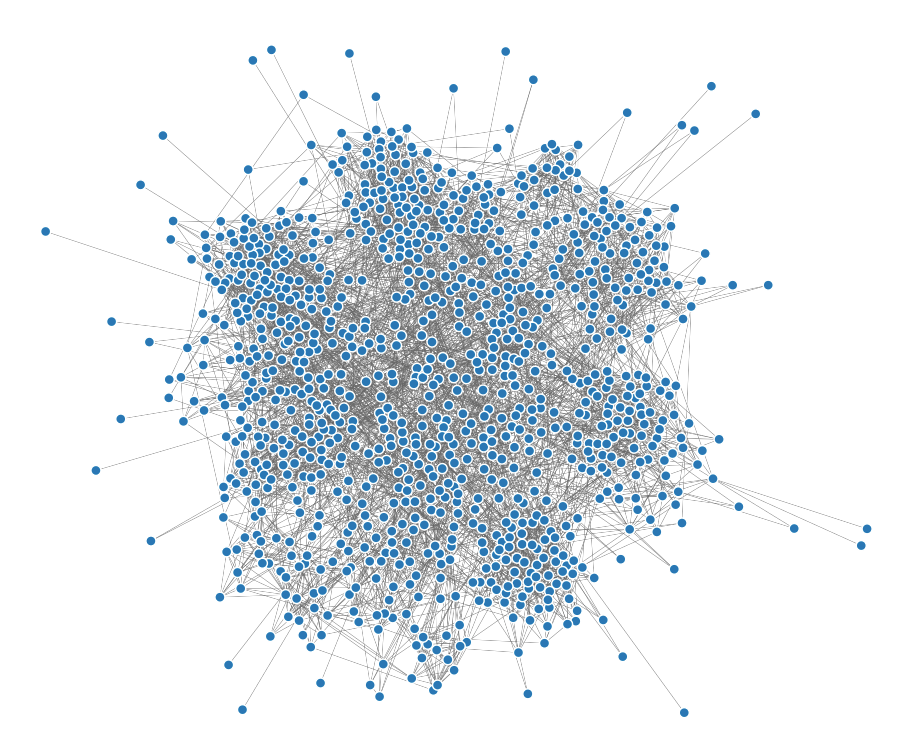
\includegraphics[width=0.75\linewidth]{images/network.png}
\end{center}

\end{textblock}

%% Column 2 ==================================================================

\begin{textblock}{0.32}(0.34,0.14)

%% Abstract ------------------------------------------------------------------

\begin{block}{Abstract \phantom{p}}

In this work, we propose \textbf{a simple yet effective solution} to the problem of
connectome inference in calcium imaging data. The proposed algorithm consists of
\textbf{two steps:
\begin{itemize}
\item[] {\color{lightgreen}i) processing the raw signals to detect neural peak activities,}
\item[] {\color{lightblue}ii) inferring the degree of association between neurons from partial
correlation statistics.}
\end{itemize}}
We summarises the methodology that led us to
win the Connectomics Challenge, proposes a simplified version of our method, and
finally compares our results with respect to other inference methods.




\end{block}



\end{textblock}

\begin{textblock}{0.32}(0.34,0.31)

%% Introduction ------------------------------------------------------------

\begin{block}{Context \phantom{p}}

Without being perfect, \textbf{calcium imaging} currently allows for \textbf{real-time and
simultaneous observation of neuron activity} from thousands of neurons,
producing \textbf{individual time-series representing their fluorescence intensity}.
From these data, the connectome inference problem amounts to retrieving the
synaptic connections between neurons on the basis of the fluorescence time-series. This problem is difficult to solve because of \textbf{experimental issues,
including
\begin{itemize}
\item[] {\color{lightgreen}i) masking effects (i.e., some of the neurons are not observed or
confounded with others),} 
\item[] {\color{lightblue}ii) the low sampling rate of the optical device with
respect to the neural activity speed,} or
\item[] {\color{lightred}iii) the slow decay of fluorescence.}
\end{itemize}}

\end{block}



\end{textblock}


%% Col 2 Row 2

\begin{textblock}{0.32}(0.34,0.525)

%% Connectome inference ------------------------------------------------------

\begin{block}{Connectome inference \phantom{p}}

Despite growing interest and practical use in various scientific areas, \textbf{variable
importances derived from tree-based ensemble methods are not well understood
from a theoretical point of view}. In this work we characterize the Mean Decrease
Impurity (MDI) variable importances as measured by an ensemble of totally
randomized trees in asymptotic sample and ensemble size conditions. \textbf{We derive a
three-level decomposition of the  information jointly provided by all input
variables about the output in terms of
\begin{itemize}
\item[] {\color{lightgreen}i) the MDI importance of each input variable,}
\item[] {\color{lightblue}ii) the degree of interaction of an input variable with the other input variables,}
\item[] {\color{lightred}iii) the different interaction terms of a given degree.}
\end{itemize}}
We then
show that this MDI importance of a variable is equal to zero if and only if the
variable is irrelevant and that the MDI importance of a relevant variable is
invariant with respect to the removal or the addition of irrelevant variables.
We illustrate these properties on a simple example and discuss how they may
change in the case of  non-totally randomized trees such as Random Forests and
Extra-Trees.

Despite growing interest and practical use in various scientific areas, \textbf{variable
importances derived from tree-based ensemble methods are not well understood
from a theoretical point of view}. In this work we characterize the Mean Decrease
Impurity (MDI) variable importances as measured by an ensemble of totally
randomized trees in asymptotic sample and ensemble size conditions. 




\end{block}


\end{textblock}


%% Col 2 Row 3

\begin{textblock}{0.32}(0.34,0.71)



\end{textblock}

%% Column 3 ==================================================================

\begin{textblock}{0.32}(0.67,0.14)

%% Experiments ---------------------------------------------------------------

\begin{block}{Experiments \phantom{p}}

Despite growing interest and practical use in various scientific areas, \textbf{variable
importances derived from tree-based ensemble methods are not well understood
from a theoretical point of view}. In this work we characterize the Mean Decrease
Impurity (MDI) variable importances as measured by an ensemble of totally
randomized trees in asymptotic sample and ensemble size conditions. \textbf{We derive a
three-level decomposition of the  information jointly provided by all input
variables about the output in terms of
\begin{itemize}
\item[] {\color{lightgreen}i) the MDI importance of each input variable,}
\item[] {\color{lightblue}ii) the degree of interaction of an input variable with the other input variables,}
\item[] {\color{lightred}iii) the different interaction terms of a given degree.}
\end{itemize}}
We then
show that this MDI importance of a variable is equal to zero if and only if the
variable is irrelevant and that the MDI importance of a relevant variable is
invariant with respect to the removal or the addition of irrelevant variables.
We illustrate these properties on a simple example and discuss how they may
change in the case of  non-totally randomized trees such as Random Forests and
Extra-Trees.

\vspace{2.5cm}

Despite growing interest and practical use in various scientific areas, \textbf{variable
importances derived from tree-based ensemble methods are not well understood
from a theoretical point of view}. In this work we characterize the Mean Decrease
Impurity (MDI) variable importances as measured by an ensemble of totally
randomized trees in asymptotic sample and ensemble size conditions. \textbf{We derive a
three-level decomposition of the  information jointly provided by all input
variables about the output in terms of
\begin{itemize}
\item[] {\color{lightgreen}i) the MDI importance of each input variable,}
\item[] {\color{lightblue}ii) the degree of interaction of an input variable with the other input variables,}
\item[] {\color{lightred}iii) the different interaction terms of a given degree.}
\end{itemize}}
We then
show that this MDI importance of a variable is equal to zero if and only if the
variable is irrelevant and that the MDI importance of a relevant variable is
invariant with respect to the removal or the addition of irrelevant variables.
We illustrate these properties on a simple example and discuss how they may
change in the case of  non-totally randomized trees such as Random Forests and
Extra-Trees.

\end{block}

\end{textblock}


%% Col 3 Row 2

\begin{textblock}{0.32}(0.67,0.42)



\end{textblock}


%% Col 3 Row 3

\begin{textblock}{0.32}(0.67,0.71)

%% Conclusion ------------------------------------------------------------

\begin{block}{Conclusion \phantom{p}}

In this paper, we outlined a simple but efficient methodology for the problem
of connectome inference from calcium imaging data. Our approach consists of \textbf{two
steps: 
\begin{itemize}
\item[] {\color{lightgreen}i) processing fluorescence data to detect neural peak activities; and}
\item[] {\color{lightblue}ii) inferring the degree of association between neurons from partial 
correlation statistics.}
\end{itemize}}

Its simplified variant outperforms other
network inference methods while its optimized version proved to be the best method
on the Connectomics Challenge. Given its simplicity and good performance, we
therefore believe that the methodology presented in this work
would constitute a solid and easily-reproducible baseline for further work in
the field of connectome inference.\\[2ex]

\textbf{Acknowledgments}\\
A. Joly and G. Louppe are research fellows of the FNRS, Belgium.  A. Sutera is a
recipient of an FRIA fellowship of FRS-FNRS, Belgium. This work is supported by
PASCAL2 and the IUAP DYSCO, initiated by the Belgian State, Science Policy
Office.


\end{block}

\end{textblock}

\end{frame}
\end{document}
